%; whizzy paragraph -pdf xpdf -latex ./whizzypdfptex.sh
%; whizzy-paragraph "^\\\\begin{frame}\\|\\\\emtext"
% latex beamer presentation.
% platex, latex-beamer でコンパイルすることを想定。 

%     Tokyo Debian Meeting resources
%     Copyright (C) 2012 Junichi Uekawa

%     This program is free software; you can redistribute it and/or modify
%     it under the terms of the GNU General Public License as published by
%     the Free Software Foundation; either version 2 of the License, or
%     (at your option) any later version.

%     This program is distributed in the hope that it will be useful,
%     but WITHOUT ANY WARRANTY; without even the implied warreanty of
%     MERCHANTABILITY or FITNESS FOR A PARTICULAR PURPOSE.  See the
%     GNU General Public License for more details.
%     You should have received a copy of the GNU General Public License
%     along with this program; if not, write to the Free Software
%     Foundation, Inc., 51 Franklin St, Fifth Floor, Boston, MA  02110-1301 USA

\documentclass[cjk,dvipdfmx,12pt]{beamer}
\usetheme{Tokyo}
\usepackage{monthlypresentation}

%  preview (shell-command (concat "evince " (replace-regexp-in-string "tex$" "pdf"(buffer-file-name)) "&")) 
%  presentation (shell-command (concat "xpdf -fullscreen " (replace-regexp-in-string "tex$" "pdf"(buffer-file-name)) "&"))
%  presentation (shell-command (concat "evince " (replace-regexp-in-string "tex$" "pdf"(buffer-file-name)) "&"))

%http://www.naney.org/diki/dk/hyperref.html
%日本語EUC系環境の時
\AtBeginDvi{\special{pdf:tounicode EUC-UCS2}}
%シフトJIS系環境の時
%\AtBeginDvi{\special{pdf:tounicode 90ms-RKSJ-UCS2}}

\newenvironment{commandlinesmall}%
{\VerbatimEnvironment
  \begin{Sbox}\begin{minipage}{1.0\hsize}\begin{fontsize}{8}{8} \begin{BVerbatim}}%
{\end{BVerbatim}\end{fontsize}\end{minipage}\end{Sbox}
  \setlength{\fboxsep}{8pt}
% start on a new paragraph

\vspace{6pt}% skip before
\fcolorbox{dancerdarkblue}{dancerlightblue}{\TheSbox}

\vspace{6pt}% skip after
}
%end of commandlinesmall

\title{東京エリアDebian勉強会}
\subtitle{第143回 2016年9月度}
\author{杉本 典充}
\date{2016年9月17日}
\logo{
\includegraphics[width=8cm]{image200607/openlogo-light.eps}}

\begin{document}

\begin{frame}
\titlepage{}
\end{frame}

\begin{frame}{Agenda}
 \begin{minipage}[t]{0.45\hsize}
  \begin{itemize}
  \item 最近あったDebian関連のイベント報告
	\begin{itemize}
	\item 第142回東京エリアDebian勉強会
	\end{itemize}
  \item 事前課題発表
  \end{itemize}
 \end{minipage}
 \begin{minipage}[t]{0.45\hsize}
  \begin{itemize}
   \item Debian Trivia Quiz
  \end{itemize}
 \end{minipage}
\end{frame}

\section{イベント報告}
\emtext{イベント報告}

\begin{frame}{第142回東京エリアDebian勉強会}

\begin{itemize}
\item 場所は朝日ネットさんをお借りして開催しました
\item 参加者は6名
\item セミナ内容は、以下内容を発表しました
  \begin{enumerate}
  \item 杉本さん「Debianでlxcをセットアップしてみよう」
  \item khibinoさん「haskell-relational-record」の紹介(飛び込み)
  \end{enumerate}
\item 残りの時間でhack timeを行い、成果発表をしました
\item \url{https://tokyodebianmeeting.titanpad.com/ep/pad/export/142/rev.487?format=txt}
\end{itemize} 
\end{frame}

\section{事前課題}
\emtext{事前課題}
{\footnotesize
 \begin{prework}{ 山下康成 }
  \begin{enumerate}
  \item 本日のHackTime作業
  \end{enumerate}
\end{prework}

\begin{prework}{ dictoss }
  \begin{enumerate}
  \item 本日のHackTime作業
  \end{enumerate}
\end{prework}

\begin{prework}{ NOKUBI Takatsugu }
  \begin{enumerate}
  \item 本日のHackTime作業
  \end{enumerate}
\end{prework}

\begin{prework}{ issei }
  \begin{enumerate}
  \item 本日のHackTime作業
  \end{enumerate}
\end{prework}

\begin{prework}{ iwamatsu }
  \begin{enumerate}
  \item 本日のHackTime作業
  \end{enumerate}
\end{prework}

\begin{prework}{ yy\_y\_ja\_jp }
  \begin{enumerate}
  \item 本日のHackTime作業
  \end{enumerate}
\end{prework}

\begin{prework}{ yosuke\_san }
  \begin{enumerate}
  \item 本日のHackTime作業
  \end{enumerate}
\end{prework}

}

\subsection{問題}

%; whizzy-master ../debianmeetingresume201311.tex
% $B0J>e$N@_Dj$r$7$F$$$k$?$a!"$3$N%U%!%$%k$G(B M-x whizzytex $B$9$k$H!"(Bwhizzytex$B$,MxMQ$G$-$^$9!#(B
%

\santaku
{debain$B%Q%C%1!<%8$N%=!<%9%3!<%I$r%@%&%s%m!<%I$9$kJ}K!$O$"$k$+<ALd$,$"$j$^$7$?!#(BDD$B$NJ}$?$A$,0FFb$7$?%5!<%S%9$O$I$l$G$7$g$&$+!#(B}
{srcs.debian.org}
{srcs.debian.net}
{sources.debian.net}
{C}
{$B4Z9q$G>pJs9)3X$r3X$s$G$$$kBg3X1!@8$NJ}$+$i%;%-%e%j%F%#$N8&5f$N0l4D$GA4%=!<%9%3!<%I$,$[$7$$$H$N$3$H$G$7$?!#$=$N$[$+$K(Bdebmirror$B%3%^%s%I$r;H$&$H$h$$$H$$$&%"%I%P%$%9$b$"$j$^$7$?!#>pJs85(B:\url{https://lists.debian.org/debian-devel/2016/09/msg00118.html}}


\section{DEP5 Machine-readable debian/copyright 再考}
\emtext{DEP5 Machine-readable debian/copyright 再考}

\begin{frame}{はじめに}

\begin{itemize}
\item  Debian ソースパッケージには debian/copyright ファイルがあり、このファイルには
対象ソフトウェアのライセンス、コピーライトが書かれている。
\item 2009年以前は特にフォーマットもなく、ライセンスも包括的な書き方。
\end{itemize}
\end{frame}

\begin{frame}[containsverbatim]{はじめに}
\begin{commandlinesmall}
gcc-defaults is Copyright (C) 2000, 2001, 2006, 2009 Debian.

These scripts are free software; you can redistribute it and/or modify it
under the terms of the GNU General Public License as published by the
Free Software Foundation; either version 2, or (at your option) any
later version.

On Debian GNU/Linux systems, the complete text of the GNU General
Public License can be found in `/usr/share/common-licenses/GPL'.

The c89 and c99 man pages are taken from netbsd:

Copyright (c) 1999 The NetBSD Foundation, Inc.
All rights reserved.
(省略)
\end{commandlinesmall}
\end{frame}

\begin{frame}{はじめに}
\begin{itemize}
\item 機械処理できるフォーマットに切り替え、自動チェックなどができるようにするため、
DEP5 / Machine-readable debian/copyright (以下、DEP5)が策定。
\item 策定後 BTS 609160 によって Debian Policy に取り込まれ、Debian Policy の一
部となる。
(Debian Policy 12.5、オプショナル扱い)
\item 最新バージョンは 1.0 であり、最新版は
\url{https://www.debian.org/doc/packaging-manuals/copyright-format/1.0/}
\end{itemize}
\end{frame}

\begin{frame}{はじめに}
\begin{itemize}
\item 多くのパッケージがDEP5 準拠の debian/copyright に切り替わっている。
\item 内容が変更されずそのまま続けるという問題がある。
\item 今回は DEP5 についてのフォーマットの紹介と、debian/copyright ファイルの更新方法について
紹介。
\end{itemize}
\end{frame}


\begin{frame}{DEP5 フォーマットについて}

\begin{itemize}
\item DEP5のフォーマット
\begin{itemize}
\item ヘッダー部 \\
  ソフトウェア全体に関わる情報、例えば頒布元や連絡先を記述
\item ファイル部 \\
  ファイル毎のコピーライトとライセンスを記述
\end{itemize}
\end{itemize}
\end{frame}

\begin{frame}{DEP5 フォーマットについて}
ヘッダー部で利用できるフィールド
\begin{itemize}
  \item Format:
  \item Upstream-Name:
  \item Upstream-Contact:
  \item Source:
  \item Disclaimer:
  \item Comment:
  \item License:
  \item Copyright:
\end{itemize}
\end{frame}

\begin{frame}{DEP5 フォーマットについて}
ファイル部で利用できるフィールド
\begin{itemize}
  \item  Files:
  \item  Copyright:
  \item  License:
  \item  Comment:
\end{itemize}
\end{frame}

\begin{frame}[containsverbatim]{DEP5 フォーマットについて}
\begin{commandlinesmall}
Files: *
Copyright: foo bar <foo@example.org>
License: GPL-2+

File: debian/*
Copyright: Nobuhiro Iwamatsu <iwamatsu@debian.org>
License: GPL-2+
 This program is free software; you can redistribute it
 and/or modify it under the terms of the GNU General Public
 License as published by the Free Software Foundation; either
 version 2 of the License, or (at your option) any later
 version.
 .
 This program is distributed in the hope that it will be
 useful, but WITHOUT ANY WARRANTY; without even the implied
 warranty of MERCHANTABILITY or FITNESS FOR A PARTICULAR
 PURPOSE.  See the GNU General Public License for more
 details.
 .
 You should have received a copy of the GNU General Public
 License along with this package; if not, write to the Free
 Software Foundation, Inc., 51 Franklin St, Fifth Floor,
 Boston, MA  02110-1301 USA
 .
 On Debian systems, the full text of the GNU General Public
 License version 2 can be found in the file
 `/usr/share/common-licenses/GPL-2'.
\end{commandlinesmall}
\end{frame}

\begin{frame}[containsverbatim]{DEP5 フォーマットについて}

その他、擬似フィールド

\begin{itemize}
\item License-Grant \\
	\debianbug{786450} 参照
\item License-Reference \\
	\debianbug{786450} 参照
\item Files-Excluded: \\
	\debianbug{685506} 参照
\end{itemize}
\end{frame}


\begin{frame}[containsverbatim]{DEP5 フォーマットについて}

erlang-cowboy パッケージの debian/copyright:
\begin{commandlinesmall}
Formats: https://www.debian.org/doc/packaging-manuals/copyright-format/1.0/
upstream-name: cowboy
upstream-contact: Loc Hoguin <essen@ninenines.eu>
Source: https://github.com/extend/cowboy.git
Files-Excluded: examples/websocket/priv/static/jquery.min.js
 examples/markdown_middleware/priv/small.mp4
 examples/markdown_middleware/priv/small.ogv
 examples/static_world/priv/small.mp4
 examples/static_world/priv/small.ogv
 examples/web_server/priv/small.mp4
 examples/web_server/priv/small.ogv

Files: *
Copyright: 2011-2012, Loc Hoguin <essen@ninenines.eu>
License: ISC

Files: debian/*
Copyright: Copyright 2012, Nobuhiro Iwamatsu <iwamatsu@debian.org>
License: Apache-2.0

License: ISC
 Permission to use, copy, modify, and/or distribute this software for any
 purpose with or without fee is hereby granted, provided that the above
 copyright notice and this permission notice appear in all copies.
 .
 THE SOFTWARE IS PROVIDED "AS IS" AND THE AUTHOR DISCLAIMS ALL WARRANTIES
 WITH REGARD TO THIS SOFTWARE INCLUDING ALL IMPLIED WARRANTIES OF
 MERCHANTABILITY AND FITNESS. IN NO EVENT SHALL THE AUTHOR BE LIABLE FOR
 ANY SPECIAL, DIRECT, INDIRECT, OR CONSEQUENTIAL DAMAGES OR ANY DAMAGES
 WHATSOEVER RESULTING FROM LOSS OF USE, DATA OR PROFITS, WHETHER IN AN
 ACTION OF CONTRACT, NEGLIGENCE OR OTHER TORTIOUS ACTION, ARISING OUT OF
 OR IN CONNECTION WITH THE USE OR PERFORMANCE OF THIS SOFTWARE.

License: Apache-2.0
 On Debian systems, the full text of the Apache License (Version 2.0)
 can be found in the file  `/usr/share/common-licenses/Apache-2.0' file.

\end{commandlinesmall}
\end{frame}

\begin{frame}{DEP5 の問題点と対策}

\begin{itemize}
\item DEP5 は ポリシーの一部であるが、オプショナル
\item 一度作ったらあまり更新しない。
\item 機械的にチェック、アップーデートできる仕組みが必要。
\end{itemize}
\end{frame}

\begin{frame}[containsverbatim]{licensecheck を使ったDEP5 フォーマット化}

licensecheck による ライセンスとコピーライトホルダーの出力

\begin{commandline}
$ licensecheck -r --copyright .
ell/io.h: LGPL (v2.1 or later)
  [Copyright: 2011-2014 Intel Corporation. All rights reserved]

ell/dbus.c: LGPL (v2.1 or later)
  [Copyright: 2011-2014 Intel Corporation. All rights reserved]
(省略)
\end{commandline}

\end{frame}

\begin{frame}[containsverbatim]{licensecheck を使ったDEP5 フォーマット化}

/usr/lib/cdbs/licensecheck2dep5 を使ったDEP5フォーマットへの整形

\begin{commandlinesmall}
$ licensecheck -r --copyright .  | /usr/lib/cdbs/licensecheck2dep5

Format: http://www.debian.org/doc/packaging-manuals/copyright-format/1.0/
Upstream-Name: FIXME
Upstream-Contact: FIXME
Source: FIXME
Disclaimer: Autogenerated by CDBS

Files: ./ell/base64.c
 ./ell/base64.h
 ./ell/checksum.c
 (中略) 
 ./unit/test-uuid.c
Copyright: 2011-2014, Intel Corporation.
  2011-2015, Intel Corporation.
  2011-2016, Intel Corporation.
  2015, Intel Corporation.
  2016, Intel Corporation.
License: LGPL (v2.1 or later)
 FIXME
(省略) 
\end{commandlinesmall}

\end{frame}

%DEP5フォーマットにして出力してくれますが、License フィールドが\texttt{FIXME}
%になっていたり、ASCII 以外の文字は文字化けするなど、完璧な出力はしてくれないため、
%生成されたテキストを修正する必要があります。

\begin{frame}[containsverbatim]{cme を使った DEP5 フォーマット化と debian/copyright の更新}

cme と libconfig-model-dpkg-perl を使ったDEP5 フォーマット化

\begin{commandlinesmall}
$ sudo apt-get install cme libconfig-model-dpkg-perl
$ cme update dpkg-copyright
cme: using Dpkg::Copyright model
updating data
(省略)
\end{commandlinesmall}

\end{frame}


\begin{frame}[containsverbatim]{cme を使った DEP5 フォーマット化と debian/copyright の更新}
c
me、libconfig-model-dpkg-perl、libconfig-model-tkui-perl パッケージによる GUI 編集

\begin{commandlinesmall}
$ sudo apt-get install libconfig-model-tkui-perl
debian/copyright を編集したい場合
$ cme edit dpkg-copyright
debian/copyright を更新した後、編集したい場合
$ cme update dpkg-copyright --edit
エディタで直接編集でも大丈夫です。
$ cme update dpkg-copyright
$ vi debian/copyright
\end{commandlinesmall}
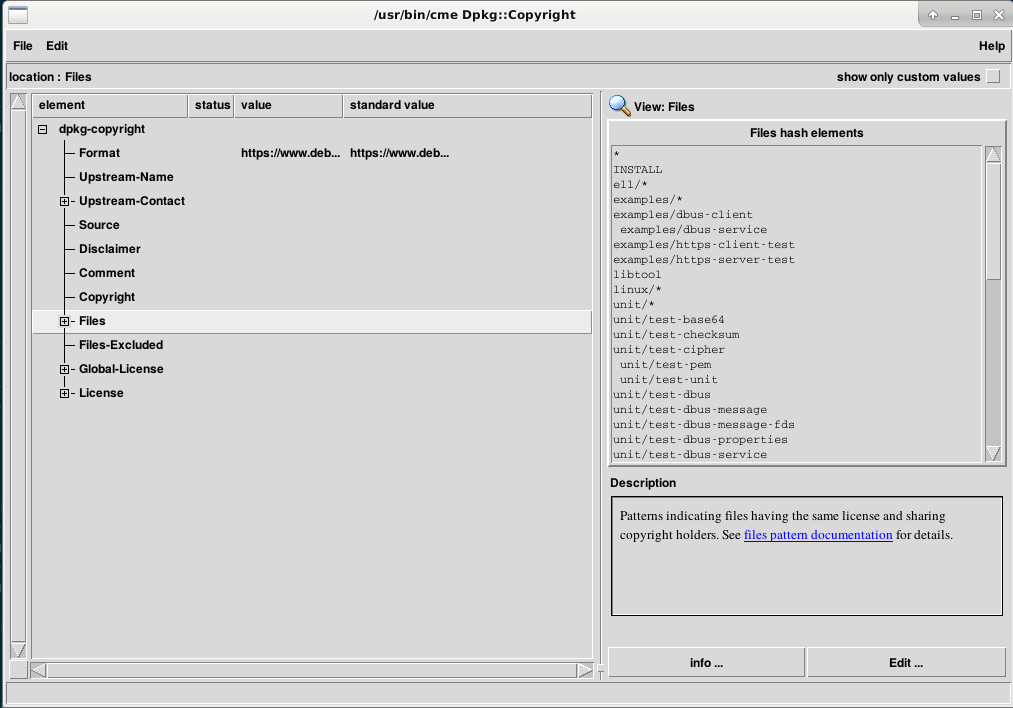
\includegraphics[width=0.7\hsize]{image201609/cme-gui.png}

\end{frame}

\begin{frame}[containsverbatim]{debmake を使った debian/copyright の DEP5フォーマット化}

debmake コマンドの \texttt{-cc} オプションを使ったDEP5フォーマット化

\begin{commandlinesmall}
$ debmake -cc > debian/copyright
\end{commandlinesmall}

\end{frame}

\begin{frame}[containsverbatim]{license-reconcile による debian/copyright チェックサポート}

license-reconcile で debian/copyright 内のチェック

\end{frame}

\begin{frame}[containsverbatim]{license-reconcile による debian/copyright チェックサポート}

debian/copyright 例:
\begin{center}
\begin{commandline}
Files: *
Copyright: 2016 foo bar <foo@example.org>
License: GPL-3+
\end{commandline}
\end{center}

debian/license-reconcile.yml 例:
\begin{commandline}
Rules:
 rules:
  -
   Glob: hoge.png
   License: GPL-2+
   Copyright: 2016 foo bar <foo@example.org>
\end{commandline}

\end{frame}

\begin{frame}[containsverbatim]{license-reconcile による debian/copyright チェックサポート}

license-reconcile 実行例:

\begin{commandline}
$ license-reconcile
License mismatch: File hoge.png has license GPL-2+ which does not match GPL-3+.\
at /usr/share/perl5/Debian/LicenseReconcile/App.pm line 222, <GEN0> line 3.
\end{commandline}

\begin{commandline}
Files: hoge.png
Copyright: foo bar <foo@example.org>
License: GPL-2+
 This program is free software: you can redistribute it and/or modify
 it under the terms of the GNU General Public License as published by
 the Free Software Foundation, either version 2 of the License, or
 (at your option) any later version.
(省略)
\end{commandline}

\end{frame}

\begin{frame}[containsverbatim]{debian パッケージ側の対応}

debian/rules にライセンスチェック用のターゲット追加による対応がお勧め。
\\
cme を使う場合:
\begin{commandlinesmall}
update-debian-copyright:
	cme update dpkg-copyright -file debian/copyright.auto
\end{commandlinesmall}

licensecheck + licensecheck2dep5 を使う場合:
\begin{commandlinesmall}
update-debian-copyright:
        licensecheck --copyright -r `find * -type f` | \
                /usr/lib/cdbs/licensecheck2dep5 > debian/copyright.auto
\end{commandlinesmall}
\end{frame}

\begin{frame}{まとめ}

\begin{itemize}
\item DEP 5 は Debian ポリシーの一部。しかしオプショナル扱い。
\item licensecheck ツールによって ソースからのライセンスとコピーライトホルダーを
抽出可能。そのままではDEP5フォーマットにならないため、licensecheck2dep5を使う。
\item cme と libconfig-model-dpkg-perl を使うことによって licensecheck +
licensecheck2dep5 同様のことが可能。岩松のお勧めはこちら。
\item license-reconcile を使うことによって cme などで補完できないファイルのチェ
ックができる。
\item 毎回 cme や licencecheck などのコマンドを実行するのではなく、debian/rules 
に書いておくとメンテナンスが楽になる。
\end{itemize}

\end{frame}

\section{Hack time}
\emtext{Hack time}

\begin{frame}{成果を記入下さい!}

  今回、Hack time時の成果を記録に残してみます。

\url{https://tokyodebianmeeting.titanpad.com/143}

に皆さんアクセス頂き(認証不要です)、各自成果を17:30までに記録するようにお願いします。

\end{frame}
  
\section{今後のイベント}
\emtext{今後のイベント}
\begin{frame}{今後のイベント}
\begin{itemize}
\item 10/15(土) 東京エリアDebian勉強会(予定)
  \begin{itemize}
  \item 発表者募集中
  \end{itemize}
\item 11/5(土),6(日) OSC 2016 Tokyo/Fall
  \begin{itemize}
  \item セミナーは11/5
  \item 展示は11/5が本番,11/6はチラシのみ
  \end{itemize}
\item 11/19(土) 東京エリアDebian勉強会(予定)
\end{itemize}
\end{frame}

\end{document}

;;; Local Variables: ***
;;; outline-regexp: "\\([ 	]*\\\\\\(documentstyle\\|documentclass\\|emtext\\|section\\|begin{frame}\\)\\*?[ 	]*[[{]\\|[]+\\)" ***
;;; End: ***
